\chapter{Routing}
\label{ch:routing}

By default the chain is serial, like the inserts of a mixer channel: the
output of each plugin feeds the next one, and the last one feeds the DAW.
The \ui{Routing} tab turns the chain into a patchbay, so that you can run
plugins in parallel, feed a sidechain from the DAW or from another plugin,
or send the outputs of a multi-output plugin to different channels.

\section{The view}

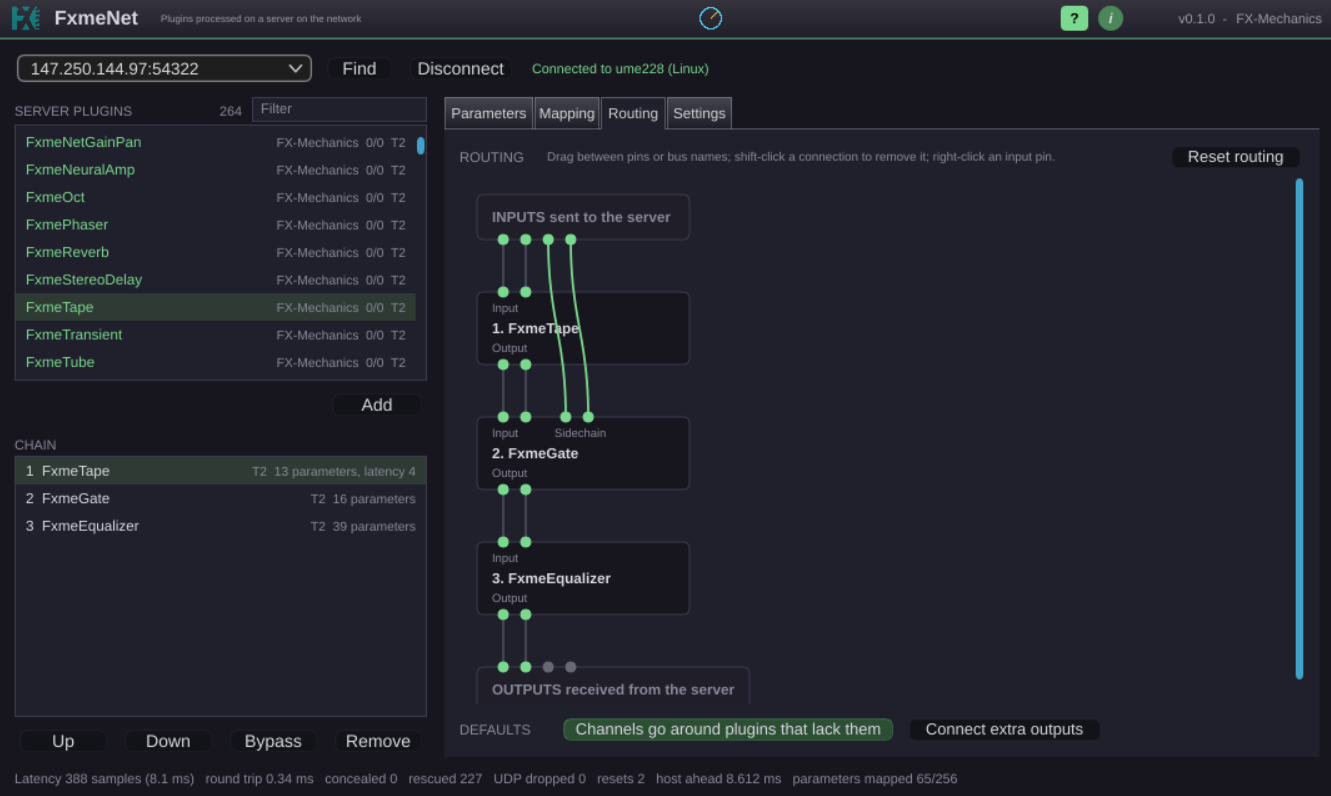
\includegraphics[width=\textwidth]{../img/fxme-net-routing-screen.png}

From top to bottom, the tab shows:

\begin{itemize}
  \item \textbf{Inputs}: the channels sent to the server (the plugin's input
    channels in the DAW);
  \item one box for each plugin of the chain, in chain order, with small
    \emph{pins} for its inputs on top and for its outputs below, grouped by
    \emph{bus} (``Main'', ``Sidechain'', and so on);
  \item \textbf{Outputs}: the channels received from the server (the plugin's
    output channels in the DAW).
\end{itemize}

A connection runs from an output pin to an input pin that is \emph{below}
it. Connections cannot go back up, so there is no feedback loop.

\section{Making and removing connections}

\begin{itemize}
  \item \textbf{Connect:} drag from an output pin to an input pin.
  \item \textbf{Connect a whole bus:} drag from a bus name to another bus
    name (or to a pin). The channels connect in order, so a stereo link
    takes one drag.
  \item \textbf{Remove:} click a connection while holding \key{Shift}.
  \item \textbf{Right-click an input pin} to disconnect it, or to put it back
    to the default rule (\ui{Back to the default routing}).
  \item \ui{Reset routing} puts the default routing back.
\end{itemize}

An output can feed several inputs (each gets a copy). Several outputs on one
input are summed, as in a DAW; this is how parallel paths are mixed back
together.

A bypassed plugin keeps its pins and passes each input channel to the output
channel with the same number.

\section{The default routing}

Until you change anything, each input of a plugin is fed by the nearest
plugin above it that has a matching output channel (the Inputs count as the
top box). This reproduces the behaviour of an ordinary serial chain:

\begin{itemize}
  \item a plugin with fewer channels than the stream lets the other channels
    pass around it to the next plugin that has them;
  \item a mono plugin with two outputs gives the plugin below its second
    output, not the DAW's second channel;
  \item sidechain and other auxiliary inputs start unconnected.
\end{itemize}

Two options under \ui{DEFAULTS} change the default rule. They never affect
connections you made by hand.

\begin{description}
  \item[Channels go around plugins that lack them] On by default. Off: each
    plugin is fed only by the one right above it, so channels that no plugin
    processes are silent.
  \item[Connect extra outputs] Off by default. On: the extra outputs of a
    plugin continue its main ones, so a plugin with two main and two extra
    outputs feeds four channels below it.
\end{description}

\section{Editing the chain after wiring}

You can add, remove and move plugins after you have wired the chain.
Connections you did not touch follow the default rule in the new chain. For
the ones you made by hand:

\begin{itemize}
  \item when a plugin is removed, what came out of it is replaced by what
    fed the same channel of its input, as if it were bypassed for good;
  \item when a plugin is moved, connections that no longer run downward are
    dropped;
  \item an input that loses all its sources through an edit goes back to the
    default, so the audio keeps flowing. An input you emptied yourself
    stays empty.
\end{itemize}

\section{Sidechains and auxiliary buses}

A sidechain input only becomes active when you connect something to it:
connect a DAW channel (an input) to the plugin's sidechain bus to compress a
bass with a kick, for example. The server then enables that bus, which
prepares that plugin again; expect a brief gap on that plugin only.
Unconnected auxiliary buses stay disabled, because many plugins behave
differently with an enabled bus that carries silence.

The channels the plugin sends to the server are the ones its connections
need. Channels you do not connect are not sent, which saves network
bandwidth.

\section{Latency and parallel paths}

When two paths of different latency meet at an input, \fxme\ delays the
shorter path so that they stay aligned. A parallel compressor, for example,
keeps its dry and wet signals in phase even when the processed path goes
through a linear-phase equaliser. The latency the DAW is told is the one of
the longest path from the inputs to the outputs.

